\documentclass[10pt,technote]{IEEEtran}
\usepackage{amssymb}
\usepackage{amsmath}
\usepackage{graphicx}
\usepackage{subcaption}

\title{Coursework 2: Representation and Distance Metrics Learning }
\author{Timothee Gathmann \textit{(\textbf{tlg15}, 01061046)}\\ Luka Lagator\textit{ ()}}

\begin{document}

\maketitle

\section{Problem formulation}
The features $X \in \mathbb{R}^{D X N}$ are readily available, and consist of a set of samples $x_i \in \mathbb{R}^D, i = 1, 2, ..., N$ corresponding to $N$ pictures of pedestrians. Each sample is assigned a ground-truth label $l(x_i) \in \mathbb{N}$ identifying the individual on the picture. The features are divided in a training subset $T$, a query subset $Q$ and a gallery subset $G$. Our goal is to minimise the retrieval error when performing retrieval experiments with the K-Nearest Neighbour algorithm \cite{Cover1967} at different ranks ($R = 1, 2, ..., 10 $), with different distance metrics. For a distance metric $d(x_i, x_j)$, the nearest neighbour $x_j \in X$ of $x_i$ is defined as
\begin{equation}
    \begin{aligned}
    n_0(x_i) = x_j \\
d(x_i, x_j) \leq d(x_i, x_n), \forall x_n \in X - x_j
    \end{aligned}
\end{equation}
The $k$ nearest neighbours of $x_i \in X$ are :
\begin{equation}
    \begin{aligned}
    n_k(x_i) = \lbrace x_j, n_{k-1}\rbrace 
    \\
    d(x_i, x_j) \leq d(x_i, x_n) \forall x_n \in X - n_k(x_i)
    \end{aligned}
\end{equation}
We define the mAp as
\begin{equation}
\begin{aligned}
    mAp & =   \frac{1}{N_Q}\sum^{N_Q}_{i, x_i \in Q}  \frac{1}{tot(x_i)}\sum^{N_G}_{j, x_j \in G}\rho(x_i, x_j)\frac{\sum^{j}_z\rho(x_i, x_z)}{j} \\ 
    tot(x_i)& = \sum^{N_G}_j\rho(x_i, x_j)
    \end{aligned}
\end{equation}
Where 
\begin{equation}
    \rho(x_i, x_z) =
    \begin{cases}
        1 & l(x_i) = l(x_z)\\
        0 & l(x_i) \neq l(x_z)
    \end{cases}
\end{equation}

It can be seen that, to minimise the mAp error, the feature space has to be transformed such that all points of same label lie the closest to each other, and all points of different labels lie the furthest from each other.
We can formulate our problem as a Distance Metric Learning problem. We define the set $S = \lbrace x_i, x_j, ...\rbrace, \rho(x_i, x_j) = 1$ and the set $D = \lbrace x_i, x_j, ...\rbrace,  \rho(x_i, x_j) = 0$
Then our problem is to solve:

\begin{equation}
\max \sum_{(x_i, x_j) \in D} d(x_i, x_j)
\end{equation}
And
\begin{equation}
\min \sum_{(x_i, x_j) \in S} d(x_i, x_j) < k, k \in \mathbb{R^+}
\end{equation}
The optimisable parameters depend on which function $d(x_i, x_j)$ is chosen, as well as which $k$ was chosen.

\section{Baseline experiments}

\subsection{Standard metrics}
The following metrics were considered as a baseline, without any transforms applied to the features:
\begin{enumerate}
    \item First order Minkowski
    \item Euclidean distance
    \item Cross Correlation similarity
    \item Cosine similarity
    \item Bilinear similarity
\end{enumerate}

We retrieved the k-nearest neighbours of the query features wit the gallery features according to each baseline metric and calculated mAp for k = 1-20. The results can be seen in the figure \ref{fig:baseline_map}. Although all metrics perform in a similar trends as the rank of the nearest neighbour algorithm is changed, the Bilinear Similarity metric and Minkowsky of order 1 metric perform better, surpassing constantly the third best performing cosine similarity by 10 percentage points. Notably, similarity metrics perform much better on  these features than classic distance metrics.
\begin{figure}
    \centering
    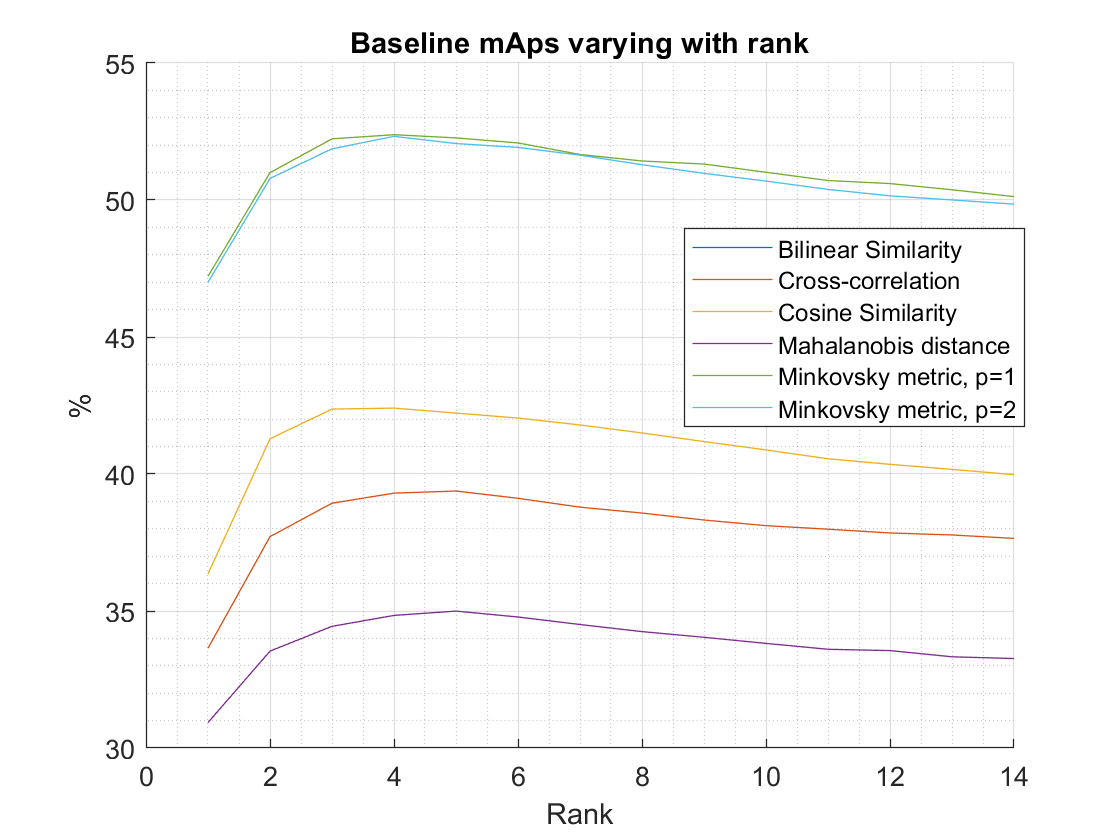
\includegraphics[width=\linewidth]{Graphs/mAp_vs_rank_baseline.png}
    \caption{Baseline mAps calculated at different ranks on testing data}
    \label{fig:baseline_map}
\end{figure}
\subsection{K-means}

\section{Improved approach: Kernel/Non-kernel Mahalanobis distance}
\subsection{}




\bibliographystyle{IEEEtran}
\bibliography{refs}
\end{document}
